\feelchapter{Heat sink}
            {Heat sink}
            {Baptiste Morin, Christophe Prud'homme}
            {cha:heatsink}

This problem considers the performance of a heat sink designed for the thermal management of high-density electronic components. The heat sink is comprised of a base/spreader which in turn supports a number of plate fins exposed to flowing air. We model the flowing air through a simple convection heat transfer coefficient. From the engineering point of view, this problem illustrates the application of conduction analysis to an important class of cooling problems: electronic components and systems. \\ \\
Our interest is in the conduction temperature distribution at the base of the spreader. The target is to study how the heat transfer occures with different parameters on our heat sink. The heat generated by high-density electronic components is such that it's very expensive to cool large structures (data center). The cooling optimization is consequent in the run for decreasing operating costs.

\noindent A classical thermal CPU cooler looks like this 

\begin{figure}[!h]
\centering
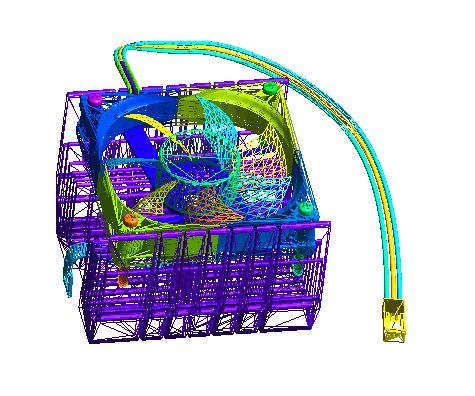
\includegraphics[width=.45\linewidth]{heatsink/complete_cooler.png}
\caption{Mesh of a classical CPU cooler}
\end{figure}

\noindent We are here going to describe how it is theorically working and how it is impleted with \feel. 

\section{Problem description}
\subsection{Domain}

We consider here a classical "radiator" which is a CPU heat sink. Those types of coolers are composed with a certain number of plate fins exposed to flowing air or exposed to a ventilator. Regarding the periodicity and geometry of our concern, we can make our study on a characteristic element of the problem : a half cell of the heat sink single thermal fin with its spreader at the basis. Let's take a look at the geometry of our problem :

\begin{figure}[!h]
\centering
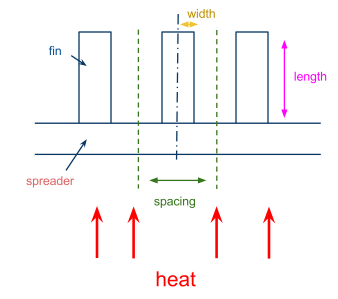
\includegraphics[width=.45\linewidth]{heatsink/sink_geom.png}
\caption{Geometry of heat sink}
\end{figure}

Our study is avaible in 2 or 3 dimensions, depending on the application's parameters. You'll see later how to work with it. Let's see on which meshes we are working on :
\begin{figure}[!h]
\begin{minipage}[b]{.50\linewidth}
\centering
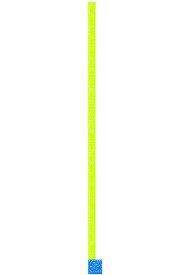
\includegraphics[width=.45\linewidth]{heatsink/mesh_2d.png}
\caption{2D mesh}
\end{minipage}
\begin{minipage}[b]{.50\linewidth}
\centering

\includegraphics[width=.65\linewidth]{heatsink/mesh_3d.png}
\caption{3D mesh}
\end{minipage}
\end{figure}

\subsection{Inputs}
The implementation of thoses parameters is described in the section ~\ref{heat:param}.

\subsubsection{Material}

Here the material parameter can be described with furthers parameters. We have, with $i=1$ for the fin and $i=2$ for the base :
\begin{itemize}
\item the thermal conductivity $\kappa_i$

\item the material's density $\rho_i$

\item the heat capacity of the material $C_i$

\end{itemize}
The term $\rho_i C_i$ corresponds to the heat volumetric capacity. In that way, we make possible the construction of a heat sink with $2$ different materials. Here is a list of the well-known ones, $\rho$ and $C$ are gave at $298 K$ :

\begin{center}
\begin{tabular}{|c|c|c|c|}
  \hline
  \textbf{Material} & \textbf{Thermal conductivity} ($\kappa$ in $W.m^{-1}.K^{-1}$) & \textbf{Density }($\rho$ in $kg.m^{-3}$) & \textbf{Heat Capacity} ($C$ in $J.kg^{-1}.K^{-1}$) \\
  \hline
  Aluminium & 180 (alloys) or 290 (pure) & 2700 & 897 \\
  \hline
  Copper & 386 & 8940 & 385 \\
  \hline
  Gold & 314 & 19320 & 129 \\
  \hline
  Silver & 406 & 10500 & 233 \\
  \hline
\end{tabular}
\end{center}

\subsubsection{Physical}
\begin{itemize}
\item{Depth} \\
This parameter is only to take into account for the 3D simulation. It represents the depth of the caracteristical heat sink and is called \lstinline!depth! in the application.

\item{Length} \\
You can also parameterize the length of the fin. This one is called \lstinline!L! in the application's parameters, its dimension is the meter.

\item{Width} \\
Typically, this parameter is linked with constructor's standards. This parameter is called \lstinline!width! in the application's implementation.
\end{itemize}

\subsubsection{Thermal}
\begin{itemize}

\item{Heat flux} \\
It represents the heat flux brought by the electronic component at the bottom of the base. Here it's typically the heat brought by the processor.

\item{Thermal coefficient} \\
The thermal coefficient $h$ named $therm_coeff$ in the application is representative of the heat transfer between the fin and the air flow. 

\item{Ambien temperature} \\
This parameter called $T_{amb}$ represents the temperature around the heat sink at the beginning. That means the ambient temperature before the computer is turned on.

\end{itemize}

\subsubsection{Summary table}
The following table displays the various fixed and variables parameters of this application.
\clearpage

\begin{table}[htbp]
  \centering
  \begin{tabular}{@{}llrrr@{}} \toprule
Name & Description & Nominal Value & Range & Units \\ \midrule
\multicolumn{2}{c}{BDF parameters} \\ \cmidrule(r){1-2}
$time-initial$ & begining & $0$ & &  \\
$time-final$ & end & $50$ & $]0, 1500]$ &  \\
$time-step$ & time step & $0.1$ & $]0,1[$ &  \\
$steady$ & steady state & $0$ & $\{0,1\}$ &  \\
$order$ & order & $2$ & $[0, 4]$ & \\\\

\multicolumn{2}{c}{Physical parameters} \\ \cmidrule(r){1-2}
$L$ & fin's length & $2\cdot 10^{-2}$ & $[0.02, 0.05]$ & $m$ \\
$width$ & fin's width & $5\cdot 10^{-4}$ & $[10^{-5}, 10^{-4}]$ & $m$ \\
$deep$ & heat sink depth & $0$ & $[0, 7\cdot 10^{-2}]$ & $m$ \\\\

\multicolumn{2}{c}{Mesh parameter} \\ \cmidrule(r){1-2}
$hsize$ & mesh's size & $10^{-4}$ & $[10^{-5},10^{-3} ]$ & \\\\

\multicolumn{2}{c}{Fin Parameters} \\ \cmidrule(r){1-2}
$\kappa_f$ & thermal conductivity & $386$ & $[100,500] $ & $W \cdot m^{-1} \cdot K^{-1}$\\
$\rho_f$ & material density & $8940$ & $[10^3,12\cdot 10^3 ]$ & $kg\cdot m^{-3}$\\
$C_f$ & heat capacity & $385$ & $[10^2,10^3]$ & $J\cdot kg^{-1} \cdot K^{-1}$\\\\

\multicolumn{2}{c}{Base/spreader Parameters} \\ \cmidrule(r){1-2}
$\kappa_s$ & thermal conductivity & $386$ & $[100,500] $ & $W \cdot m^{-1} \cdot K^{-1}$\\
$\rho_s$ & material density & $8940$ & $[10^3,12\cdot 10^3 ]$ & $kg\cdot m^{-3}$\\
$C_s$ & heat capacity & $385$ & $[10^2,10^3]$ & $J\cdot kg^{-1} \cdot K^{-1}$\\\\

\multicolumn{2}{c}{Heat Parameters} \\ \cmidrule(r){1-2}
$T_{amb}$ & ambient temperature & $300$ & [300,310] & $K$ \\
$heat\_flux$ & heat flux $Q$ & $10^6$ & $[0 ,10^{6}]$ & $W \cdot m^{-3}$\\
$therm\_coeff$ & thermal coefficient $h$ & $10^3$ & $[0,10^3]$ & $W\cdot m^{-2} \cdot K^{-1}$ \\
\end{tabular}

  \caption{Table of fixed and variable parameters}
  \label{tab:param}
\end{table}


\section{Theory}
\label{therm:equations}

\subsection{Figure}
The global domain is $\varOmega = \varOmega_1 \cup \varOmega_2 $ where $\varOmega_1$ is the fin's domain and $\varOmega_2$ the spreader's domain. We note $\partial\varOmega$ the border of the domain $\varOmega$. The physical lines we are using will be noted as $\Gamma_i$ such as described above. The following figure describes the parameters and the geometry we are using in the equations to solve our 3D issue :
The following figures describe the parameters and the geometry we are using in the equations to solve our 2D or 3D issue :
\begin{figure}[!h]
\centering
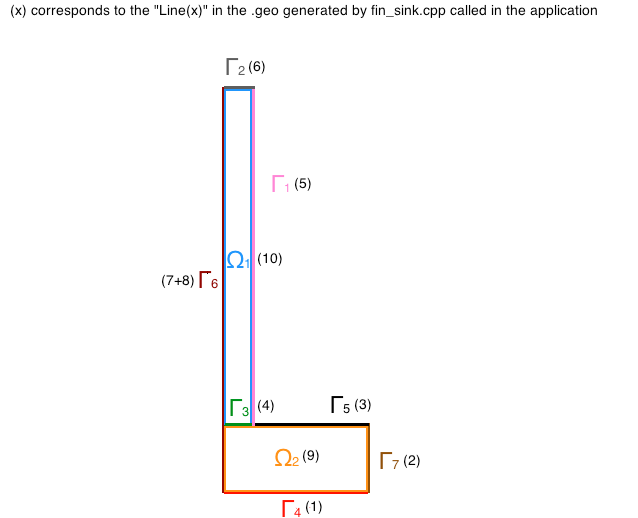
\includegraphics[width=.50\linewidth]{heatsink/figure_2d.png}
\caption{2D geometry details}
\end{figure}

\begin{figure}[!h]
\centering
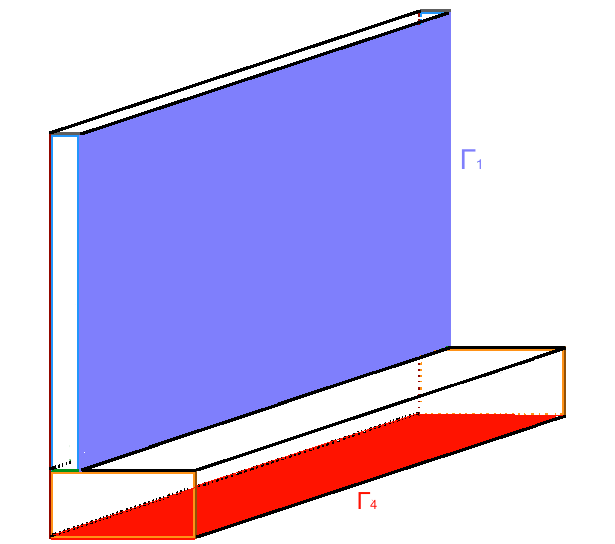
\includegraphics[width=.50\linewidth]{heatsink/figure_3d.png}
\caption{3D geometry details}
\end{figure}
\clearpage

\subsection{Equations}

Our concern satisfies the heat equation which reads 
\begin{equation}
\label{heat:eq}
   \begin{split}
      \displaystyle{\sum_{i=1}^{2} \kappa_i \Delta T - \rho_i C_i \frac{ \partial T}{\partial t}}  & = 0
  \end{split}
\end{equation}
\begin{equation}
\label{hom_neu1}
   \begin{split}
      \displaystyle{ \kappa_1 \frac{\partial T}{\partial n}} & =  0 \quad on \quad \Gamma_2 \quad and \quad \Gamma_6 \\ \\ 
  \end{split}
\end{equation}
\begin{equation}
\label{hom_neu2}
   \begin{split}
      \displaystyle{ \kappa_2 \frac{\partial T}{\partial n}} & =  0 \quad on \quad \Gamma_5 , \Gamma_7 \quad and \quad \Gamma_8 \\ \\ 
  \end{split}
\end{equation}
\begin{equation}
\label{classic_neu}
   \begin{split}
      \displaystyle{ \kappa_1 \frac{\partial T}{\partial n}} & = - h( T - T_{amb}) \quad on \quad \Gamma_1 \\ \\
  \end{split}
\end{equation}
\begin{equation}
\label{nonhom_neu}
   \begin{split}
      \displaystyle{ \kappa_2 \frac{\partial T}{\partial n}} & =  Q(1-e^{-t}) \quad on \quad \Gamma_4 \\ \\
  \end{split}
\end{equation}
\begin{equation}
\label{temp_conti}
   \begin{split}
      T_{| \varOmega_1} & = T_{| \varOmega_2} \quad on \quad \Gamma_3 \\ \\
  \end{split}
\end{equation}
\begin{equation}
\label{flux_conti}
   \begin{split}
      \displaystyle{ \kappa_1 \nabla T \cdot n} & = \displaystyle{ \kappa_2 \nabla T \cdot n \quad on \quad \Gamma_3} \\ \\
  \end{split}
\end{equation}

\noindent with $i=1$ for the fin and $i=2$ for the base and where $\kappa_i$ is the thermal conductivity, $\rho_i$ is the material's density ($kg.m^{-3}$ in the SI unit), $C_i$ the heat capacity and $T$ the temperature at a precise point (in 2D or 3D). To see how it has been coded, you can read \ref{heat:eq_impl}.


\subsection{Boundary conditions}
\label{heat:bc}
The problem requieres that the temperature and heat flux are continute on $\Gamma_3$. Considering the problem's geometry, we also impose zero heat flux on the vertical surfaces of the spreader. Let's detail the conditions we have imposed :
\begin{itemize}
\item Homogeneous Neumann condition (\ref{hom_neu1}) and (\ref{hom_neu2}) : it represents the fact that the heat flux is only vertical (for $\Gamma_6$ and $\Gamma_7$) or the fact that the heat flux is only provided by $\Gamma_4$ (for $\Gamma_2$ and $\Gamma_5$).

\item Homogeneous Neumann condition (\ref{classic_neu}) : it imposes that the heat flux is brought by this surface (it mathematically represents that the heat sink is placed on the heat source).

\item Non-homogeneous Neumann condition (\ref{nonhom_neu}) :  this boundary condition represents the transient state for the heat transfer calculation.

\item Temperature continuity (\ref{temp_conti}) : it imposes that the temperature is continute at the interface between the two materials (if there are two materials, we can also have the same one for the two pieces).

\item Heat flux continuity (\ref{flux_conti}) : it represents that the heat flux is continute at the interface between the two materials. Literally, it means that the two flows offset each other.

\end{itemize}

\noindent Theses conditions have been coded as explained in the section \ref{heat:eq_impl}.

\subsection{Finite Element Method}
Let's apply the method to our concern, we introduce the test function $v$ and we integrate the main equation, which reads now as :
\begin{equation}
   \begin{split}
      \displaystyle{\sum_{i=1}^{2} \rho_i C_i \int_{\varOmega_i} v\frac{ \partial T}{\partial t} - \kappa_i \int_{\varOmega_i} v\Delta T }  & = 0  
  \end{split}
\end{equation}
We integrate by parts, which leads to :
\begin{equation}
   \begin{split}
      \displaystyle{\sum_{i=1}^{2} \rho_i C_i \int_{\varOmega_i} v\frac{ \partial T}{\partial t} +  \kappa_i \int_{\varOmega_i} {\nabla v \cdot \nabla T} - \kappa_i \int_{\partial \varOmega_i} {(\nabla T \cdot n) v} }  & = 0
  \end{split}
\end{equation}
then, by decomposing the borders $\partial\varOmega_i$, we obtain :
\begin{multline}
 \displaystyle{- \kappa_1 \int_{\Gamma_1}{(\nabla T \cdot n) v} - \kappa_2 \int_{\Gamma_4} {(\nabla T \cdot n) v} - \kappa_1 \int_{\Gamma_{2,6}}{(\nabla T \cdot n) v}  - \kappa_2 \int_{\Gamma_{5,7,8}}{(\nabla T \cdot n) v} } \quad + \\ \displaystyle{ \sum_{i=1}^{2}  \rho_i C_i \int_{\varOmega_i} v\frac{ \partial T}{\partial t} + \kappa_i \int_{\varOmega_i} {\nabla v \cdot \nabla T} - \kappa_i \int_{\partial\varOmega_i \cap \Gamma_3}{(\nabla T \cdot n) v}  } =   0 
\end{multline}
Now, we apply the conditions (\ref{hom_neu1}), (\ref{hom_neu2}), (\ref{classic_neu}) and (\ref{nonhom_neu}) which brings us to :
\begin{equation}
   \begin{split}
 \displaystyle{ \int_{\Gamma_1}{hv(T-T_{amb})} - \int_{\Gamma_4} {vQ(1-e^{-t})} + \sum_{i=1}^{2}  \rho_i C_i \int_{\varOmega_i} v\frac{ \partial T}{\partial t} + \kappa_i \int_{\varOmega_i} {\nabla v \cdot \nabla T}  - \underbrace{\kappa_i \int_{\partial\varOmega_i \cap \Gamma_3}{(\nabla T \cdot n) v}}_{\text{=0 thanks to \ref{flux_conti}}}  } & =   0 
  \end{split}
\end{equation}
Now we apply the boundary conditions (\ref{flux_conti}) which results in :
\begin{equation}
   \begin{split}
 \displaystyle{ h \int_{\Gamma_1}{v(T-T_{amb})} - \int_{\Gamma_4} {vQ(1-e^{-t})}  + \sum_{i=1}^{2} \rho_i C_i \int_{\varOmega_i} v\frac{ \partial T}{\partial t} + \kappa_i \int_{\varOmega_i} {\nabla v \cdot \nabla T} } & =   0 
  \end{split}
\end{equation}
We can now start to transform the equation by puting in the right hand the known terms :
\begin{equation}
   \begin{split}
 \displaystyle{ h \int_{\Gamma_1}{v T}  + \sum_{i=1}^{2} \rho_i C_i \int_{\varOmega_i} v\frac{ \partial T}{\partial t} + \kappa_i \int_{\varOmega_i} {\nabla v \cdot \nabla T} } & =  
 \int_{\Gamma_4} {vQ(1-e^{-t})}	 +  hT_{amb}\int_{\Gamma_1}{v}
  \end{split}
\end{equation}
We discretize $\displaystyle{\frac{\partial T}{\partial t}}$ where $\delta t$ is the time step, such as:
\begin{equation}
   \begin{split}
 \displaystyle{ h \int_{\Gamma_1}{v T} + \sum_{i=1}^{2} \rho_i C_i \int_{\varOmega_i} v\frac{T^{n+1} - T^n}{\delta t} + \kappa_i \int_{\varOmega_i} {\nabla v \cdot \nabla T} } & =  
 \int_{\Gamma_4} {vQ(1-e^{-t})}	 +  hT_{amb}\int_{\Gamma_1}{v}
  \end{split}
\end{equation}
Finally we obtain :
\begin{equation}
\color{red}
   \begin{split}
 \displaystyle{ h \int_{\Gamma_1}{v T} + \sum_{i=1}^{2} \rho_i C_i \int_{\varOmega_i} v\frac{T^{n+1}}{\delta t} + \kappa_i \int_{\varOmega_i} {\nabla v \cdot \nabla T}} & =  
	\displaystyle{ \int_{\Gamma_4} {vQ(1-e^{-t})} +  hT_{amb}\int_{\Gamma_1}{v}	+  \sum_{i=1}^{2}  \rho_i C_i \int_{\varOmega_i} v \frac{T^n}{\delta t}  }
  \end{split}
\end{equation}
This is that equation which is implemented in the application \lstinline!feel_heatsink!.

\section{Implementation}
\label{heat:impl}

\subsection{Application parameters}
\label{heat:param}

The parameters of the application are implemented such as 
\begin{lstlisting}
inline
Feel::po::options_description
makeOptions()
{
Feel::po::options_description heatsinkoptions("heatsink options");
heatsinkoptions.add_options()
// mesh parameters
("hsize", Feel::po::value<double>()->default_value( 0.1 ),
 "first h value to start convergence")
("L", Feel::po::value<double>()->default_value( 0.03 ),
 "dimensional length of the sink (in meters)")
("width", Feel::po::value<double>()->default_value( 0.0005 ),
 "dimensional width of the fin (in meters)")

// 3D parameter
("deep", Feel::po::value<double>()->default_value( 0 ),
 "depth of the mesh (in meters) only in 3D simulation")

// thermal conductivities parameters
("kappa_s", Feel::po::value<double>()->default_value( 386 ),
 "thermal conductivity of the base spreader in SI unit W.m^{-1}.K^{-1}")
("kappa_f", Feel::po::value<double>()->default_value( 386 ),
 "thermal conductivity of the fin in SI unit W.m^{-1}.K^{-1}")

// density parameter
("rho_s", Feel::po::value<int>()->default_value( 8940 ),
 "density of the spreader's material in SI unit kg.m^{-3}")
("rho_f", Feel::po::value<int>()->default_value( 8940 ),
 "density of the fin's material in SI unit kg.m^{-3}")

// heat capacities parameter
("c_s", Feel::po::value<double>()->default_value( 385 ),
 "heat capacity of the spreader's material in SI unit J.kg^{-1}.K^{-1}")
("c_f", Feel::po::value<double>()->default_value( 385 ),
 "heat capacity of the fin's material in SI unit J.kg^{-1}.K^{-1}")

// physical coeff
("therm_coeff", Feel::po::value<double>()->default_value(50),
 "thermal coefficient")
("Tamb", Feel::po::value<double>()->default_value(300),
 "ambiant temperature")
("heat_flux", Feel::po::value<double>()->default_value(1e6),
 "heat flux generated by CPU")

("steady", Feel::po::value<bool>()->default_value(false), 
 "if true : steady else unsteady")

// export
("export-matlab", "export matrix and vectors in matlab" );

return heatsinkoptions.add( Feel::feel_options() );
}
\end{lstlisting}

\subsection{Surfaces}

To be able to calculate the surfaces in further dimension without changing the code, we have given the same names for the faces we were interested in. In 2D $\Gamma_i$ represents a line whereas in 3D it represents a surface. The calculation of those surfaces which makes possible the calculation of averages temperature is as follow :
\begin{lstlisting}
surface_base = 
 integrate( _range= markedfaces(mesh,"gamma4"), _expr= cst(1.)).evaluate()(0,0);

surface_fin = 
 integrate( _range= markedfaces(mesh,"gamma1"), _expr=cst(1.)).evaluate()(0,0);
\end{lstlisting}

\subsection{Equations}
\label{heat:eq_impl}
First we start by calculate the non-steady state which means that we integrate all the time-independant terms, which is done with :
\begin{lstlisting}
/*
 * Right hand side construction (steady state)
 */
form1( _test=Xh, _vector=F, _init=true ) = 
 integrate( _range= markedfaces(mesh, "gamma1"), _expr= therm_coeff*Tamb*id(v));

/*
 * Left hand side construction (steady state)
 */
form2( Xh, Xh, D, _init=true ) = 
integrate( _range= markedelements(mesh,"spreader_mesh"), 
		_expr= kappa_s*gradt(T)*trans(grad(v)) );

form2( Xh, Xh, D) += 
integrate( _range= markedelements(mesh,"fin_mesh"), 
		_expr= kappa_f*gradt(T)*trans(grad(v)) );

form2 (Xh, Xh, D) += 
integrate( _range= markedfaces(mesh, "gamma1"), 
		_expr= therm_coeff*idt(T)*id(v));

form2(Xh, Xh, D) +=
  integrate( _range=markedelements(mesh, "spreader_mesh"), 
	      	_expr=rho_s*c_s*idt(T)*id(v)*M_bdf->polyDerivCoefficient(0) )
  + integrate( _range=markedelements(mesh, "fin_mesh"), 
		_expr=rho_f*c_f*idt(T)*id(v)*M_bdf->polyDerivCoefficient(0) );
\end{lstlisting}

Then, to compute the transient state, which means time dependant terms, you have to initialize the temperature (which is initialized as $T_{amb}$ on $X_h$ space) and create a new vector  $F_t$ which corresponds to the time dependent term. The code is as follow :
\begin{lstlisting}
T = vf::project( _space=Xh, _expr=cst(Tamb) );
M_bdf->initialize(T);
auto Ft = M_backend->newVector( Xh );

for ( M_bdf->start(); M_bdf->isFinished()==false; M_bdf->next() )
{
        // update right hand side with time dependent terms                                                                                              
        auto bdf_poly = M_bdf->polyDeriv();
        form1( _test=Xh, _vector=Ft ) =
            integrate( _range=markedelements(mesh, "spreader_mesh"), 
			  _expr=rho_s*c_s*idv(bdf_poly)*id(v)) +
            integrate( _range=markedelements(mesh, "fin_mesh"), 
			 _expr=rho_f*c_f*idv(bdf_poly)*id(v) );
			
        form1( _test=Xh, _vector=Ft ) +=
            integrate( _range= markedfaces(mesh,"gamma4"),
			 _expr= heat_flux*(1-exp(-M_bdf->time()))*id(v) );

        // add contrib from time independent terms                                                                                                       
        Ft->add( 1., F );

        // solve 
        M_backend->solve( _matrix=D, _solution=T, _rhs=Ft );

        // both average temperatures
        Tavg = integrate( _range=markedfaces(mesh,"gamma4"), 
			_expr=(1/surface_base)*idv(T) ).evaluate()(0,0);
				
        Tgamma1 = integrate( _range=markedfaces(mesh,"gamma1"), 
			_expr=(1/surface_fin)*idv(T) ).evaluate()(0,0);

        // export results                                                                                                                                
        out << M_bdf->time() << " " << Tavg << " " << Tgamma1 << "\n";

        this->exportResults( M_bdf->time(), T );

}
\end{lstlisting}

\subsection{Outputs}
As you can see in the equation's implementation above, there are two ouputs :
\begin{itemize}
\item \textsc{Gmsh} format : this file contains the entire mesh and the temperatures associated to each degrees of freedom of the mesh. To open it, you juste have to do as you always do with \textsc{Gmsh} : \lstinline!gmsh heatsink-1_0.msh!. You will obtain the figure with the different temperatures, you are now able to click on "play" with its significative logo and admire the evolution

\item \lstinline!averages! file : this file is completed at each time step, each line contains the current time, the average temperature on $\Gamma_4$ (surface where is the contact between the heat sink and the heat source) and the average temperature on $\Gamma_1$. To analyze this file, we recommend you to work with \textsc{Octave} which is an open-source software similar to \textsc{Matlab}. If it is installed, open a command line and go to \lstinline!~/feel/heatsink/Simplex_*.*.*/0.000*/! and try :
\begin{lstlisting}
> octave
octave:1> M=load('averages');
octave:2> plot(M(:,1),M(:,2))
octave:3> plot(M(:,1),M(:,3))
octave:4> plot(M(1:70,1),M(1:70,2))
octave:5> plot(M(1:70,1),M(1:70,3))
\end{lstlisting}

The $4^{th}$ and $5^{th}$ lines are here to observe the transient state.
\end{itemize}


\section{Use cases}
\subsection{How to use it ?}
To make easier the use of this application, we recommand you to use the configurations files. This is the fastest way : to do it, you juste have to create the file \lstinline!heatsink.cfg! and place it in the same directory that your application's executable. \\
We have created $3$ typical \lstinline!cfg! files such as :
\begin{lstlisting}
# file heatsink_1.cfg
# spreader and fin in copper
# 2D simulation
hsize=1e-4

kappa_s=386 # W/m/K                                                                                                                                      
c_s=385
rho_s=8940

kappa_f=386 # W/m/K                                                                                                                                      
c_f=385 #J/kg/K                                                                                                                                          
rho_f=8940

L=15e-3
width=5e-4                                                                                                                                               

therm_coeff=1000  #W/(m2K)                                                                                                                               
heat_flux=1e6

[bdf]
order=2
time-step=0.05
time-final=100
steady=0

[exporter]
format=gmsh
\end{lstlisting}

\begin{lstlisting}
# file heatsink_3.cfg
# spreader in copper
# fin in aluminium
# 3D simulation
hsize=3e-4
kappa_s=386 # W/m/K                                                                                                                                      
c_s=385
rho_s=8940

kappa_f=386 # W/m/K                                                                                                                                      
c_f=385 #J/kg/K                                                                                                                                          
rho_f=8940

L=15e-3
width=5e-4
deep=4e-2

therm_coeff=1000  #W/(m2K)                                                                                                                               
heat_flux=1e6

[bdf]
order=2
time-step=0.05
time-final=100
steady=0

[exporter]
format=gmsh
\end{lstlisting}

This file is the only modification you will have to bring to the application, in that way you won't have to compile each time the files (except for \lstinline!heatsink.cpp! if you want to increase the order and/or the dimension, in that case you'ill have to modify this parameter at then end of the file in the \lstinline!main! method).

\subsection{Results}

\subsubsection{2D cases}
Here are some results of the 2D simulations considering different configurations files. The figures have been extracted thanks to \textsc{Gmsh} and \textsc{Octave} :

\begin{figure}[!h]
\centering
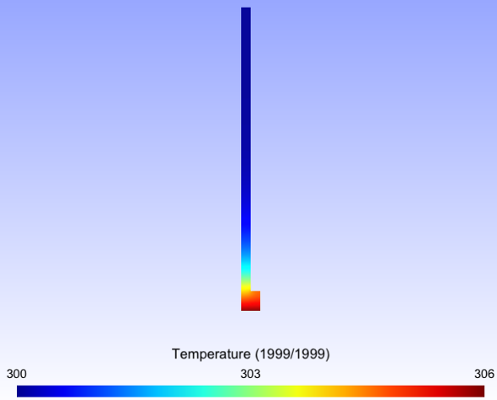
\includegraphics[width=10cm]{heatsink/heatsink_1.png}
\caption{\lstinline!heatsink_1.cfg! : steady state, spreader and fin in copper, $Q=1e6$ and $h=1e3$}
\end{figure}


\begin{figure}[!h]
\begin{minipage}[b]{.5\linewidth}
\centering
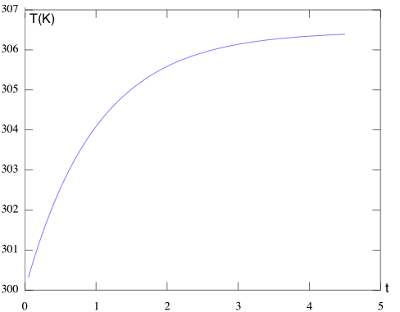
\includegraphics[width=7cm]{heatsink/heatsink_1_gamma4.png}
\caption{\lstinline!heatsink_1.cfg! : transient state on $\Gamma_4$}
\end{minipage}
\begin{minipage}[b]{.5\linewidth}
\centering
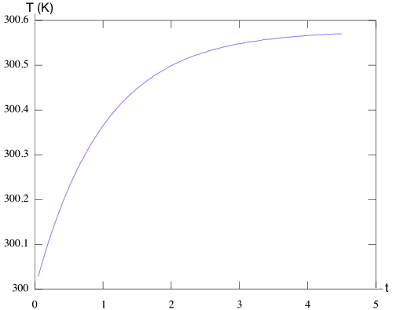
\includegraphics[width=7cm]{heatsink/heatsink_1_gamma1.png}
\caption{\lstinline!heatsink_1.cfg! : transient state on $\Gamma_1$}
\end{minipage}
\end{figure}

\clearpage

%\item \lstinline!heatsink_2.cfg! : spreader and fin in copper, $Q=1e8$ and $h=20$
%\begin{figure}[!h]
%\centering
%\includegraphics[width=1.7cm]{heatsink/heatsink_2.png}
%\end{figure}

\subsubsection{3D cases}
Here is the result of 3D simulations considering the following configurations :

\begin{figure}[!h]
\centering
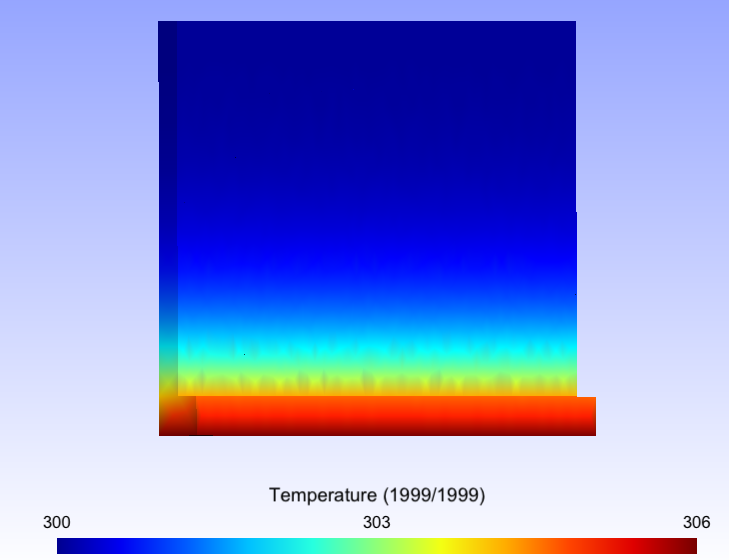
\includegraphics[width=10cm]{heatsink/heatsink_3.png}
\caption{\lstinline!heatsink_3.cfg! : spreader and fin in copper, $Q=1e6$ and $h=1e3$}
\end{figure}

\begin{figure}[!h]
\begin{minipage}[b]{.5\linewidth}
\centering
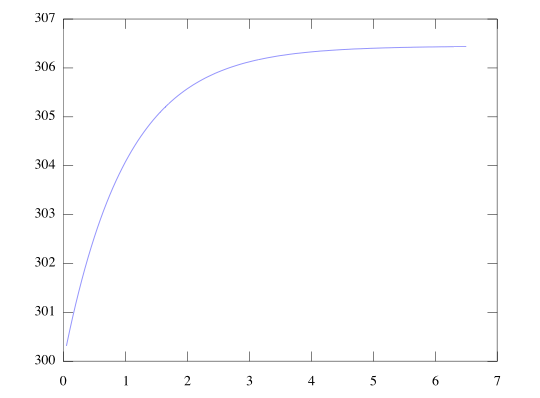
\includegraphics[width=7cm]{heatsink/heatsink_3_gamma4.png}
\caption{\lstinline!heatsink_3.cfg! : transient state on $\Gamma_4$}
\end{minipage}
\begin{minipage}[b]{.5\linewidth}
\centering
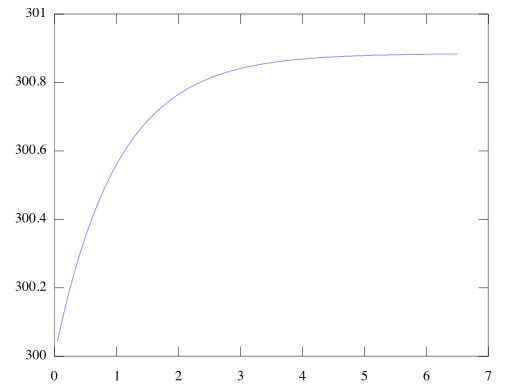
\includegraphics[width=7cm]{heatsink/heatsink_3_gamma1.png}
\caption{\lstinline!heatsink_3.cfg! : transient state on $\Gamma_1$}
\end{minipage}
\end{figure}


%\item \lstinline!heatsink_4.cfg! : spreader in copper and fin in aluminium, $Q=1e8$ and $h=20$
%\begin{figure}[!h]
%\centering
%\includegraphics[width=9cm]{heatsink/heatsink_4.png}
%\caption{Steady state}
%\end{figure}

\clearpage